\documentclass[12pt]{article}
\usepackage{lmodern}
\usepackage{amssymb,amsmath}
\usepackage{natbib} %bibliography package

\usepackage{setspace}
\doublespacing


\usepackage{ifxetex,ifluatex}
\usepackage{fixltx2e} % provides \textsubscript
\ifnum 0\ifxetex 1\fi\ifluatex 1\fi=0 % if pdftex
  \usepackage[T1]{fontenc}
  \usepackage[utf8]{inputenc}
\else % if luatex or xelatex
  \ifxetex
    \usepackage{mathspec}
  \else
    \usepackage{fontspec}
  \fi
  \defaultfontfeatures{Ligatures=TeX,Scale=MatchLowercase}
  \newcommand{\euro}{€}
\fi
% use upquote if available, for straight quotes in verbatim environments
\IfFileExists{upquote.sty}{\usepackage{upquote}}{}
% use microtype if available
\IfFileExists{microtype.sty}{%
\usepackage{microtype}
\UseMicrotypeSet[protrusion]{basicmath} % disable protrusion for tt fonts
}{}
\usepackage[margin=1in]{geometry}
\usepackage{hyperref}
\PassOptionsToPackage{usenames,dvipsnames}{color} % color is loaded by hyperref
\hypersetup{unicode=true,
            pdftitle={The Effect of Recycled Individuals in the Jolly-Seber Model with Tag Loss},
            pdfborder={0 0 0},
            breaklinks=true}
\urlstyle{same}  % don't use monospace font for urls
\usepackage{graphicx,grffile}
\makeatletter
\def\maxwidth{\ifdim\Gin@nat@width>\linewidth\linewidth\else\Gin@nat@width\fi}
\def\maxheight{\ifdim\Gin@nat@height>\textheight\textheight\else\Gin@nat@height\fi}
\makeatother
% Scale images if necessary, so that they will not overflow the page
% margins by default, and it is still possible to overwrite the defaults
% using explicit options in \includegraphics[width, height, ...]{}
\setkeys{Gin}{width=\maxwidth,height=\maxheight,keepaspectratio}
\setlength{\parindent}{0pt}
\setlength{\parskip}{6pt plus 2pt minus 1pt}
\setlength{\emergencystretch}{3em}  % prevent overfull lines
\providecommand{\tightlist}{%
  \setlength{\itemsep}{0pt}\setlength{\parskip}{0pt}}
\setcounter{secnumdepth}{0}

%%% Use protect on footnotes to avoid problems with footnotes in titles
\let\rmarkdownfootnote\footnote%
\def\footnote{\protect\rmarkdownfootnote}

%%% Change title format to be more compact
\usepackage{titling}

% Create subtitle command for use in maketitle
\newcommand{\subtitle}[1]{
  \posttitle{
    \begin{center}\large#1\end{center}
    }
}

\setlength{\droptitle}{-2em}
  \title{The Effect of Recycled Individuals in the Jolly-Seber Model with Tag
Loss}
  \pretitle{\vspace{\droptitle}\centering\huge}
  \posttitle{\par}
  
  %Remove Authors for blind submssion
%  \author{Emily Malcolm-White\textsuperscript{1},
%        Laura L.E. Cowen\textsuperscript{2}, 
%        Clive R. McMahon\textsuperscript{3}\\ 
%        \textsuperscript{1} Academic Assistance and Tutoring, University of California Davis, Davis, CA, USA\\ 
%        \textsuperscript{2} Department of Mathematics and Statistics, University of Victoria, Victoria, BC, Canada\\
  %      \textsuperscript{3} Sydney Institute for Marine Science, Mosman, NSW, Australia}



% Uncomment DATE for submssion to remove date
  \date{}
%  \predate{}\postdate{}



% Redefines (sub)paragraphs to behave more like sections
\ifx\paragraph\undefined\else
\let\oldparagraph\paragraph
\renewcommand{\paragraph}[1]{\oldparagraph{#1}\mbox{}}
\fi
\ifx\subparagraph\undefined\else
\let\oldsubparagraph\subparagraph
\renewcommand{\subparagraph}[1]{\oldsubparagraph{#1}\mbox{}}
\fi

\begin{document}
\maketitle


\begin{quote}
\textsc{Summary:} In capture-recapture studies, recycled individuals occur
when individuals lose all of their tags and are recaptured as though they were new
individuals. Typically, the effect of these recycled individuals is
assumed negligible. Through a simulation-based study, we examine the
effect of recycled individuals on parameter estimates in the
Jolly-Seber model with tag loss \citep{Cowen:2006} in double tagging experiments. With low tag-retention
rates, high capture rates, and high survival rates, recycled individuals
can produce overestimates of population size. These results are
particularly noticeable in longer studies. We validate the simulation
framework using long-term census data of elephant seals where we found population size estimates to be between 8 and 53\% larger when recycled individuals were ignored. However, including recycled individuals did not affect estimates of capture, survival, and tag-retention probabilities.
\end{quote}

\begin{quote}
\begin{center} \textsc{Key words:} Abundance; Capture-mark-recapture; Complete tag loss; Demography; Double-tagging; Elephant seal. 
\end{center}
\end{quote}

\section{Introduction}\label{introduction}

Mark-recapture studies utilize statistical techniques to estimate
population parameters. Over \(k\) sampling
periods, individuals are captured, tagged with unique tags, released and potentially
recaptured at subsequent sampling times. The Jolly-Seber (JS) model \citep{Jolly:1965, Seber:1965}
 is used to model open populations since it
can estimate parameters of interest such as population size and survival
rates \citep{Pollock:1990}. An important assumption of this model is that 
individuals never lose their tags. However, when this assumption is
violated, serious bias can occur in the parameter and variance estimates
\citep{Arnason:1981}. Double-tagging, the placement of two tags on
an individual, can be used to estimate tag retention rates. Double tagging studies have been used for a wide variety of species (for example cod: \citealt{Bjornsson:2011}, lobsters: \citealt{Xu:2014}:, sea turtles: \citealt{Bjorndal:1996}, elephant seals: \citealt{Pistorius:2000}, black bears: \citealt{Diefenbach:1998})   to investigate probabilities of tag loss or tag shedding rates.  Often a
mixture of single- and double-tagged individuals is used for practical
purposes. \cite{Cowen:2006} incorporated tag-loss by developing
the Jolly-Seber tag-loss (JSTL) model for experiments where some
fraction of individuals are double tagged. This model was further
extended to account for heterogeneity in capture between groups \citep{Xu:2014}. In the simplest form of the JSTL model, it is assumed that
every individual present in the population at sampling occasion \(k\)
has capture, survival, and tag retention
probabilities that are homogeneous for all individuals in the population
across all sampling occasions.  However, these assumptions are rarely met and can induce significant bias in the parameter estimates \citep{Schwarz:2012}.

Occasionally in mark-recapture experiments, previously captured
individuals lose all of their tags (complete tag loss). These
individuals are either recognized upon recapture (for example, through
scarring or fin clipping), and not re-tagged, or if unrecognized, these
individuals would be tagged again and treated as ``new'' individuals.
Individuals who lose both tags and are recaptured and re-tagged are
known as recycled individuals. For example, an individual with the
following tag history over three sampling occasions \{11 01 00\} was
double tagged at time 1, lost a tag between times 1 and 2, and may have
lost it's last tag between sampling occasions 2 and 3 and then have been
recaptured at sampling occasion 3 resulting in a new individual with
capture history \{00 00 11\}. If the rate of tag loss is small, bias in
the population estimate will also be small for the Peterson estimators
\citep{Seber:1981}. Typically in the JS and JSTL models, the
effect of recycled individuals is assumed to be negligible. However, in
situations where tag retention is low and survival and recapture
probabilities are high it is suspected that recycled individuals will
bias population size estimates upwards. The motivation for this study
was to investigate the effect of recycled individuals on parameter
estimates in the JSTL model through a simulation study and determine
under which conditions researchers need to be concerned.  This study is important as the assumption that the effect is negligible has not been fully tested and quantified, and most studies that rely on marking individuals typically experience tag loss. Thus, there is a need to account for recycled individuals given the desire for accurate and robust estimates for management and conservation purposes.

In order to determine whether the simulation framework provided a
reasonable approximation to the real world, we analyzed the effects of
recycled individuals in long-term census data of elephant seals (\textit{Mirounga leonina}). For
this particular population, seals could be identified even if they lost
both tags given that they had a permanent brand \citep{McMahonWhite:2009}.

\section{Methods}\label{methods}

\subsection{The Jolly-Seber Model with Tag Loss
(JSTL)}\label{the-jolly-seber-model-with-tag-loss-jstl}

Full development of the JSTL model is given by \citep{Cowen:2006} and summarized in the Online Supplement including a table of notation.  

Many different models can be specified for the JSTL model where
parameters are homogeneous or heterogeneous with respect to time or
group. We consider the case of the JSTL model where capture, survival,
and tag retention probabilities are constant over time \citep{Cowen:2006}.

Assumptions of the JSTL model with constant survival, capture, and tag
retention probabilities and time-varying entry probabilities are as
follows:

\begin{itemize}
\tightlist
\item
  The effect of recycled individuals is negligible
\item
  All individuals (marked and unmarked) are equally catchable, and that
  capture probabilities for all individuals are the same for all
  individuals at all sample times
\item
  All individuals (marked and unmarked) have equal survival
  probabilities between all sample times
\item
  All individuals have equal entry (birth or immigration) probabilities,
  but entry probabilities can vary between sample times
\item
  All marked individuals have equal tag retention probabilities between
  all sample times
\item
  For double-tagged individuals, tag loss is independent between tags
\item
  There is independence across all individuals
\item
  The sampling period is relatively short compared to the interval
  between sampling times
\end{itemize}

\subsubsection{Likelihood and
Estimation}\label{likelihood-and-estimation}
The JSTL model is developed under the idea of a superpopulation (the number of individuals that will enter population at some point during the study) \citep{Schwarz:1996} and this allows the likelihood to be formulated into three parts: 1) a model for the observed number of unique tag histories given the superpopulation size ($L_1^A$), 2) a model for the recaptures given the observed number of unique tag histories ($L_1^B$), and 3) a model for the number of individuals lost on capture ($L_3$).  The third component $L_3$, is typically used for harvest or fisheries data when known deaths occur.  In this study and in the elephant seal application, we assume there is no possibility of loss on capture, thus the third component of the likelihood simplifies to 1. The
full likelihood is given by the product of the components of the
likelihood (\(L=L_1^A \times L_1^B\)) and can be found in the Online Supplement.

Maximum likelihood parameter estimates are found using a Newton-Raphson type
method. Estimated standard errors are computed using the delta theorem.
Models were implemented using R software \citep{R}, and code can be obtained from the second author.

\subsection{Experimental Design}\label{experimental-design}

To study the effect of recycled individuals on parameter estimates of
this model, we conducted a simulation study. Data were simulated and
analyzed using R 3.1.1 \citep{R}. Data sets varied both in super-population size,
parameter values and percent double tagged. We generated data for the
JSTL model with constant survival, capture, and tag retention
probabilities for a double-tagging experiment. Super-population sizes of
1000 and 100 000 were considered in order to determine the effect that
population size may have on the results. For the super-population size
of 100 000, experiments with ten sampling occasions were considered. For
the super-population size of 1000 we considered experiments with five,
seven and ten sampling occasions in order to determine if the length of
the study has any effect on the results. For each population size, we
tested different proportions of double-tagged versus single-tagged
individuals (\(0.5\) and \(1\)). Survival, capture, and tag retention
probability parameters were varied in a \(3^3\) experimental design with
low (\(0.2\)), medium (\(0.5\)) and high (\(0.9\)) values for each
parameters. The entry rates were fixed to be $1/k$ at each of the
sampling times. No individuals were lost on capture.

We considered the set of parameter values to be reasonable values that might be encountered in practice and also produce informative capture-recapture scenarios.  Tag retention rates can vary by species, age of the tag, tag type, tag location, behaviour, season, and individual quality (size of an animal for example in seals).  For example, tag retention rates have ranged from 13\% \citep{Fogarty:1980} to 95\% \citep{Gonzalez:2012} in lobsters.  Other studies report tag retention rates of 65\% male elephant seals \citep{Pistorius:2000} and 88\% in Adelie penguins \citep{Ainley:1980}.  Mean retention of visible implant tags has been recorded as 32\% in small rockpool fish \citep{Griffiths:2002}. Turtles in particular experience high tag loss rates.  For example \cite{Bellini:2001} reports the probability of tag loss in hawksbill turtles as 0.57 and    \cite{Bjorndal:1996} observed the probability of tag loss  in green nesting turtles to be as high as 0.38.   Thus, we chose a wide range of tag loss parameter values to try to capture the diversity among published tag loss rates.

\subsubsection{Simulation of Data}\label{simulation-of-data}

For all of the parameter combinations of super-population size
(\(N=1 000, 100 \ 000\)), fraction double-tagged (\(0.5, 1\)), survival
probability (\(\phi=0.2,0.5,0.9\)), capture probability
(\(p=0.2,0.5,0.9\)) and tag retention probability
(\(\Lambda=0.2,0.5,0.9\)), we generated 100 data sets where the
simulated data met all the assumptions of the model.

For each individual, we simulated a capture history using the following
algorithm:

\begin{enumerate}
\def\labelenumi{\arabic{enumi}.}
\item
  Determine when the individual enters the population utilizing the
  entry probabilities.
\item
  For each time period after entry (until death or first capture) 
  determine if the individual survives to that time period (with
  probability \(\phi\)). If they are still alive, determine if they were
  first captured (with probability \(p\)). If they are captured,
  determine whether they are single or double-tagged.
\item
  For each time period after first capture (until death, loss of all
  tags or the end of the study) determine if the individual survives to
  that time period (with probability \(\phi\)). Then if they are still
  alive, determine if they lose any of their tags (with probability
  \(1-\Lambda\)). If they still have at least one of their tags,
  determine if they were recaptured (with probability \(p\)). If they
  have lost all of their tags, consider them as a new individual
  entering the population at this time period.
\end{enumerate}

By keeping track of all the recycled individuals, this algorithm 
provides us with two data sets: one that includes the recycled
individuals (assumes individuals, who have lost their tags, are tagged
again upon recapture and treated as new individuals) and one that
doesn't include recycled individuals (assumes that individuals, who
have lost their tags, can be recognized upon recapture and are not
re-tagged). The JSTL model was fit to the 100 simulated data sets twice
(once with and once without recycled individuals). We assumed that any
difference between the two analyses was due entirely to the recycled
individuals.

\subsubsection{Evaluation Criteria}\label{evaluation-criteria}

To evaluate the resulting parameter estimates from each of the simulations, we looked at several criteria including: average parameter
estimate, relative bias of the estimates, the average standard error of
the parameter estimates, the standard deviation of the parameter
estimates, and root mean squared error (RMSE) of the parameter
estimates.

Given that the \(\hat{p_i}\)'s are the parameter estimates from each of
the 100 simulations, we calculated:

\begin{itemize}
\tightlist
\item
  the mean parameter estimate as
  \(\hat{p}= \frac{1}{100} \sum_{i=1}^{100} \hat{p_i}\)
\item
  average standard error of the parameter estimate as
  \(\text{SE}(\hat{p})= \frac{1}{100} \sum_{i=1}^{100} \text{SE}(\hat{p_i})\).
\item
  the standard deviation of the parameter estimates as
  \(\text{SD}(\hat{p})= \sqrt{\frac{1}{99} \sum_{i=1}^{100} (\hat{p_i}-\hat{p})^2}\).
\item
  the RMSE of the parameter estimates as
  \(\text{RMSE}= \sqrt{\frac{1}{100} \sum_{i=1}^{100} (\hat{p_i}-p)^2} \approx \sqrt{\hat{\text{SD}}^2+\hat{\text{Bias}}^2}\).
\end{itemize}

We compared the average parameter estimates  to the true parameter
values using relative bias. We calculated the relative bias of the
estimators as \(\left(\hat{p}\right) =(\hat{p} -p)/p\), where
\(\hat{p}\) is the average parameter estimate calculated from the 100
simulations and \(p\) is the true value of the parameter. We also
compared the relative bias from the analysis with the recycled
individuals to the relative bias from the analysis without the recycled
individuals. We calculated the difference in the two relative biases and
consider this to be the relative bias that was contributed entirely by the
recycled individuals being tagged as ``new'' individuals.




\section{Simulation Results}\label{results}

The relative bias of the survival estimates are biased for some
parameter combinations of survival, capture, and tag retention
probabilities. As an example, box plots of survival estimates for data
with super-population size N=1000 and 100\% double tagging are provided
(Figure 1). Box plots of survival estimates for other super-population
sizes and double-tagging rates are provided in the Online Supplement (Figures
A1-A4). Although there is bias in the survival estimates for several of
the parameter combinations, the bias is similar between the analysis
with and the analysis without the recycled individuals included for both
super-population sizes (\(N=1000\) and \(100 000\)) and for both
double-tagging rates (\(T_2=0.5,1\)). In fact, the differences in
relative bias due to recycled individuals for the parameters \(\phi\),
\(p\) and \(\Lambda\) is small (\textless{}0.01) for all 108 parameter
combinations considered. In general, the SE, SD and RMSE of the
estimates of \(\phi\), \(p\) and \(\Lambda\) are similar for both the
analysis with and without recycled individuals for the parameter
combinations considered. It seems that, in general, the treatment of
recycled individuals has little effect, if any, on the accuracy of the
JSTL estimators for survival, capture, and tag-retention probabilities.
Box plots of capture and tag retention estimates for all models can also
be found in the Online Supplement (Figures A5-A12).

Results are similar for both the super-population sizes of 1000 and
100000 for all parameter combinations of survival, capture, and tag
retention probabilities. There is slightly more bias due to recycled
individuals for parameter combinations where the probability of double
tagging (\(T_2\)) was only 0.5, compared to the parameter combinations
where all individuals were double tagged. As an example, relative bias of
the parameters are presented for the parameter combination where
\(\phi=0.9, p=0.9\) and \(\Lambda=0.2\) for both the analysis with and
without recycled individuals for varying population size and
double-tagging probabilities (Table 1).

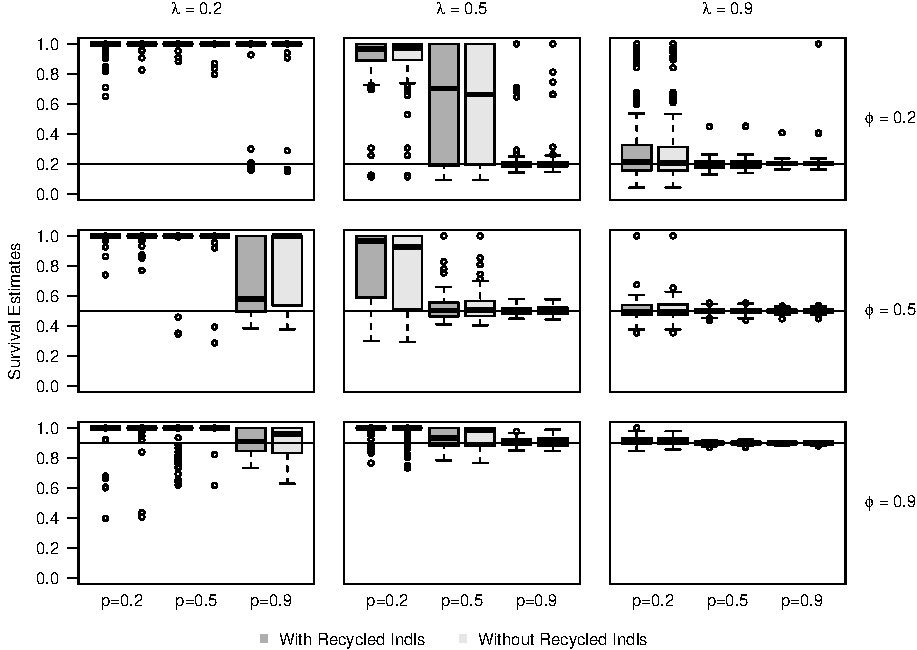
\includegraphics{RecycledPaper_files/figure-latex/Figure1_survival_GJSTL1-1.pdf}

\begin{quote}
\textsc{Figure 1:}
\textsl{Survival probability estimates for simulated data with super-population size $N=1000$ with 100\% double-tagging for different tag retention probabilities ($\Lambda=0.2,0.5,0.9$), survival probabilities ($\phi=0.2,0.5,0.9$), and different capture probabilities ($p=0.2,0.5,0.9$) using the JSTL model from a ten-sample-time study. Box plots of the estimates of $\phi$ for the model analyzed with and without the recycled individuals are provided. The black line indicates the true value of $\phi$ used to simulate the data for each model.}
\end{quote}

~ ~

\begin{quote}
\textsc{Table 1:}
\textsl{The mean relative bias of the parameters from the model analyzed with ($R$) and without ($R'$) the recycled individuals for data with high survival probability ($\phi=0.9$), high capture probability ($p=0.9$), and low tag retention ($\Lambda=0.2$)  for different super-populations sizes ($N=1000,100 000$) and different tag retention probabilities ($T_2=0.5,1$) using the JSTL model from a ten-sample-time study. }
\end{quote}

\begin{table}[ht]
\centering
\begin{tabular}{rcccccccc}
  \hline
  & \multicolumn{8}{l}{Population Size ($N$) and Proportion Double Tagged ($T_2$)} \\
  \cline{2-9}
  & \multicolumn{4}{l}{N=1000} & \multicolumn{4}{l}{N=100000} \\
  \cline {2-9}
 & $T_2=1$ && $T_2=0.5$ && $T_2=1$ && $T_2=0.5$ &  \\ 
  \cline {2-9}
  & $R$ & $R'$ & $R$ & $R'$ & $R$ & $R'$ & $R$ & $R'$ \\ 
  \hline
$\phi$ & 0.00 & 0.00 & 0.06 & 0.05 & 0.00 & 0.00 & 0.11 & 0.10 \\ 
  p & 0.00 & 0.00 & 0.00 & 0.00 & 0.00 & 0.00 & 0.00 & 0.00 \\ 
  $\Lambda$ & 0.00 & 0.00 & 0.00 & 0.00 & 0.00 & 0.00 & -0.09 & -0.08 \\ 
  N & 1.98 & 0.00 & 2.13 & 0.00 & 1.98 & 0.00 & 2.12 & 0.00 \\ 
   \hline
\end{tabular}
\end{table}

~ ~

The estimate of super-population size (\(\hat{N}\)) is computed as
\(\hat{N}=n_{\text{obs}}/{(1-\hat{P}_0)}\), where \(\hat{P}_0\) is the
estimated probability of never being seen. In the scenarios where many
recycled individuals were recaptured and considered as ``new''
individuals, the number of observed individuals, \(n_{\text{obs}}\), is larger than it should  be and thus,
\(\hat{N}\) is biased upwards. This bias is corrected in the analysis
without the recycled individuals considered. The relative bias in the
super-population size (\(\hat{N}\)) due to recycled individuals is 
highest in the scenario with high survival rates (\(\phi=0.9\)), high
capture rates (\(p=0.9\)) and low tag retention rates (\(\Lambda=0.2\)),
as predicted (Figure 2, Table 1). The relative bias is small for all
scenarios where tag retention was high, but relative bias increases as
tag retention decreases. The relative bias in \(\hat{N}\) decreases as
capture probability decreases, but recycled individuals appear to still
have some effect on the estimates even when capture probabilities
are low (\(p=0.2\)). The relative bias in \(\hat{N}\) is high for
scenarios where survival probability is high, and decreases as
survival probability decreases. In all scenarios where survival probability is
low (\(\phi=0.2\)) individuals are unlikely to survive long enough to be
able to be tagged, lose tag(s) and be recaptured as  ``new''
individuals. When survival probability is low, the relative bias due to the recycled
individuals is small (less than 0.15) and hence not shown in Figure 2.
SE, SD, and RMSE of \(\hat{N}\) varies, but remains similar between the
analyses with and without recycled individuals included, across all
scenarios.

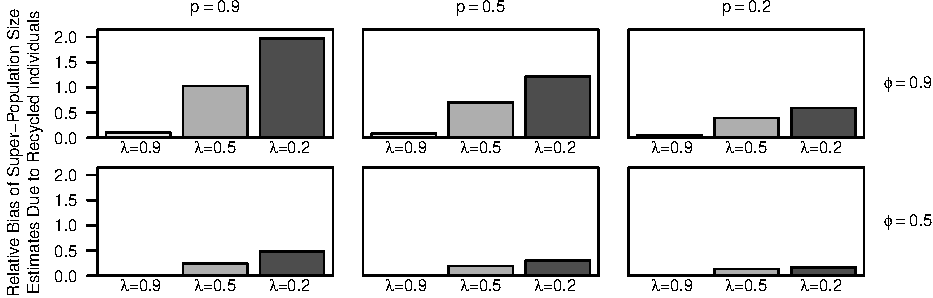
\includegraphics{RecycledPaper_files/figure-latex/Figure2_N-1.pdf}

\begin{quote}
\textsc{Figure 2:}
\textsl{The difference in mean relative bias of the super-population estimate ($\hat{N}$) between the model analyzed with and without the recycled individuals for data with super-population size $N=100 000$ with 100\% double-tagging for different tag retention probabilities ($\Lambda=0.2,0.5,0.9$), survival probabilities ($\phi=0.2,0.5,0.9$), and capture probabilities ($p=0.2,0.5,0.9$) using the JSTL model from a ten-sample-time study.}
\end{quote}

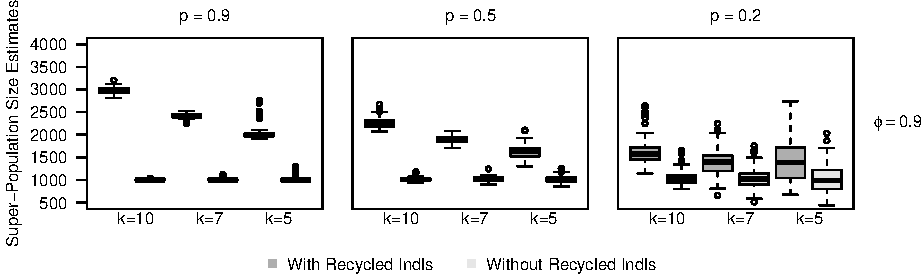
\includegraphics{RecycledPaper_files/figure-latex/Figure3_N_k-1.pdf}

\begin{quote}
\textsc{Figure 3:}
\textsl{Box plots of the estimates of $N$ for the model analyzed with and without the recycled individuals for data with super-population size $N=1000$ with 100\% double-tagging for different capture probabilities ($p=0.2,0.5,0.9$), and constant survival ($\phi=0.9$) and tag retention ($\Lambda=0.2$) probabilities using the JSTL model from experiments with $k=10, 7,$ and $5$ sample-times. }
\end{quote}

There is more bias in \(\hat{N}\) due to recycled individuals in longer
experiments (Figure 3). With a larger number of sampling occasions,
there is more time for individuals to be captured and tagged, lose their
tags, and survive to be recaptured (be recycled). In shorter studies,
there are fewer numbers of recycled individuals and thus the bias in
\(\hat{N}\) due to recycled individuals is lower although not
unnoticeable in the worst case scenarios (low tag retention, high
survival and high capture probabilities). Box plots of super-population
size (\(N\)) for all scenarios are available in the Online Supplement (Figures
A19-A24).

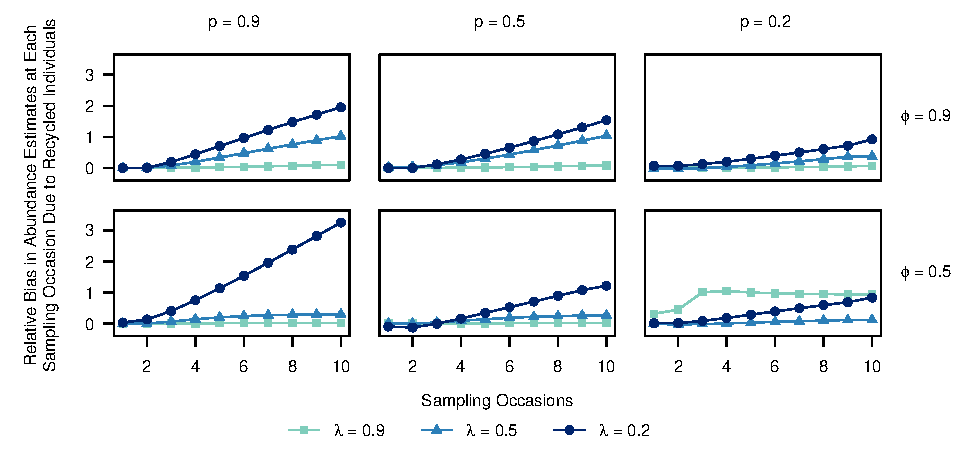
\includegraphics{RecycledPaper_files/figure-latex/Figure4_N_j-1.pdf}

\begin{quote}
\textsc{Figure 4:}
\textsl{The difference in mean relative bias of the abundance estimates at each time period ($\hat{N_j}$) between the model analyzed with and without the recycled individuals for data with super-population size N=100 000 with 100\% double-tagging for different tag retention probabilities ($\Lambda=0.2,0.5,0.9$), survival probabilities ($\phi=0.2,0.5,0.9$), and different capture probabilities ($p=0.2,0.5,0.9$) using the JSTL model from a ten-sample-time study.  Note that lines are added between the points to emphasize the difference in values; no models were fit to generate these lines.}
\end{quote}

In general, the bias due to recycled individuals in the \(\hat{N}_j\)'s
follows a similar pattern to the bias due to recycled individuals in
\(\hat{N}\), with relative bias in the \(\hat{N}_j\)'s increasing as tag
retention decreases, survival increases, and capture probability
increases (Figure 4). For all scenarios, the relative bias in the
estimates of abundance at each sample time \(j\) is smaller for earlier
sampling occasions and larger for later sampling occasions. Since the
estimates of the population sizes at each time \(j\) are computed
iteratively as
\(\hat{N}_{j+1}=\hat{\phi}(\hat{N_j})+\hat{b_j}(\hat{N})\), any bias in
the earlier abundance estimates is magnified in the later sampling
occasions abundance estimates. The scenario with \(\phi=0.5\),
\(p=0.9\), and \(\Lambda=0.2\) appears to have very high relative bias
in the abundance estimates in later sampling occasions (\textgreater{}3
for \(\hat{N}_{10}\)), which is caused by a combination of more upward
bias in the survival probability estimates for the analysis with recycled
individuals than without (Figure A14) as well as upward bias in the
super-population size estimates. Plots of the mean abundance estimates
for all scenarios are available in the Online Supplement (Figures A17-A28).

\subsection{Case Study: Elephant
Seals}\label{case-study-elephant-seals-1}


To validate the simulation framework, we analyzed data from a long-term mark-recapture study of elephant seals on Macquarie Island. The data
used for the case study consists of 7 years between 1993 and 2000.
Elephant seal pups were marked with two tags in the inter-digital
webbing of their hind flippers and were given a permanent hot-iron
branding with a unique identifier on their flank \citep{McMahon:2009}. This
permanent branding allowed for individual elephant seals to be
identified even if they lost both tags. Thus, recycled individuals could
be easily identified.

We considered two analyzes of the data:

\begin{enumerate}
\def\labelenumi{\arabic{enumi}.}
\item
  We assumed that recycled individuals could not be recognized upon
  recapture (ignoring branding) and were re-tagged as if they are new
  individuals. This scenario simulates analysis ignoring the effects of
  recycled individuals.
\item
  Recycled individuals were recognized upon recapture (by branding) and were re-tagged with new tags identical to their lost tags.
\end{enumerate}


For the elephant seal data, there were several differences in parameter
estimates of the JSTL model when recycled individuals were included
compared to when recycled individuals were excluded. For this analysis, we used the same model as the simulation study where capture, survival and tag retention rates were held constant.  

As expected, the
super-population size estimate for the analysis which included the
recycled individuals ($\hat{N}=8985$) is 30\% larger than the estimate in the analysis
which excluded recycled individuals ($\hat{N}=6949$) who were recognized upon recapture. This relationship also holds true for the abundance estimates
at each time period (Table 2). The bias in the abundance estimates increases
 as time goes on, again validating the results of our
simulation study.

Similar to the simulations, there is not much difference in the
estimates of survival and capture probabilities between the analysis
with and without recycled individuals. For comparison to the previous
simulations, we note that tag retention probability for the
elephant seals was estimated to be $\approx 0.8$ (high).  Standard error estimates are also higher when recycled individuals are included in the analysis. 

\begin{quote}
\textsc{Table 2}
\textsl{Estimates of survival probability ($\phi$), capture probability ($p$), and super-population size ($N$) for the elephant seal data analyzed with and without the recycled individuals. Standard errors are presented for survival and capture probabilities.}
\end{quote}

\begin{center}
\begin{tabular}{c c c c c}
& \multicolumn{2}{l}{With Recycled} & \multicolumn{2}{l}{Without Recycled} \\ \hline
Parameter & Estimate & SE & Estimate & SE \\ \hline
$\phi$ & 0.759 & 0.006 & 0.744 & 0.006\\
$p$ & 0.682 & 0.006 & 0.741 & 0.006 \\
$\Lambda $ & 0.792 & 0.005 & 0.799 & 0.005\\ \hline
%$N$ & 8985 & & 6949& \\ \hline
$N_{1994}$ & 1740 & 48 & 1601 & 36 \\
$N_{1995}$ & 1859 & 41 & 1717 & 40 \\
$N_{1996}$ & 2515 & 46 & 2264 & 42 \\
$N_{1997}$ & 3179 & 50 & 2727 & 43 \\
$N_{1998}$ & 3793 & 54 & 2965 & 48 \\
$N_{1999}$ & 4300 & 59 & 3229 & 46 \\
$N_{2000}$ & 4973 & 65 & 3238 & 50 \\ \hline
\end{tabular}
\end{center}

\section{Discussion}\label{discussion}
Through both a simulation study and an elephant seal case study, we examined the effect of recycled individuals on parameter estimates from the Jolly-Seber tag loss model.
In an attempt to emulate the many different real life scenarios
researchers may face, we simulated over many different values of
survival probability, capture probability, tag-retention probability, population size, study length, and proportion double tagged. While
these scenarios do not cover all possible realistic mark-recapture
experiments, our simulations are sufficient to show that the JSTL
abundance estimates can be substantially biased by recycled individuals,
especially when tag-retention is low combined with high survival, high
capture rates, or both. This effect is especially noticeable in longer
experiments. These results brings context to the assumption that the effect of
recycled individuals is negligible in mark-recapture models. However, we
show that in general, recycled individuals have little effect on the
accuracy of the survival, capture, and tag-retention probability
estimates and that for short-term studies, the effects are reduced.

Although the case study of elephant seals validated some of the results from
the simulation study (recycled individuals bias abundance estimates
upwards), some caution must be taken when comparing simulation studies
to the real world. There are many parameters that may differ or be
uncertain, such as entry probabilities, that may influence the results.
Simplifications of the individuals in the simulation studies may not
take into account the complexities that arise in real life
scenarios.

Although our study provides some evidence that recycled individuals have
an effect on estimators of the JSTL model in particular situations,
there is room for improvement in our approach and questions remain for
future work. We only examined three levels of survival, capture, and
tag-retention probabilities (Low=0.2, Medium=0.5 and High=0.9) which was
intended to simulate across a variety of scenarios that may exist
in real life. Future work could examine levels of survival, capture, or
tag retention for scenarios of interest for particular populations or
could simulate across more levels to try to get a better sense of the
relationship between the parameters and the effect of recycled
individuals. Additionally, future work could examine the effect of
recycled individuals in situations where survival, capture or
tag-retention probabilities are thought to be time-varying.

For researchers interested in conducting and analyzing mark-recapture
studies, unsurprisingly we stress the importance of using tags with high retention
rates, especially in situations where survival and capture rates are
suspected to be high. As long as tag-retention is high, the JSTL
estimator of population size is not affected by recycled individuals. In
situations where it is possible to recognize if an individual has been
captured previously (by scarring, marking, etc), excluding these
recycled individuals from the analysis can improve accuracy of the
abundance estimates. Permanent marking should be used where possible. If
researchers are only interested in the survival rates, they do not need
to be concerned with the effect of recycled individuals regardless of
the study's tag-retention rates.

Developing a model to incorporate recycled individuals is a similar problem to that of incorporating misidentification of individuals.  \cite{Schwarz:1999} developed a model to deal with tag-misreads in an open population capture-recapture setting.  However most of the misidentification literature focusses on genetic or photographic identification errors.  Here multiple identities can be assigned to the same individual leading to overestimates in population size if misidentification is ignored \citep{Yoshizaki:2011}. This is the same result that we see when recycled individuals are ignored.   \cite{Link:2010} introduced the notion of using a latent multinomial to model the latent capture histories for a closed population model. Others have extended \citeauthor{Link:2010}'s model to deal with multiple non-invasive marks \citep{Bonner:2013, McClintock:2013}, heterogeneity in parameters \citep{Mcclintock:2014} and open populations \citep{Bonner:2013}.  These latent multinomial models could be extended to include misidentification produced by complete tag loss.

Finally, the JSTL model we looked at did not include a component for loss on capture (when for example a fishery harvest occurs).  It would be interesting for future work to include loss on capture to determine if recycled individuals are still problematic under this scenario.  There remains a great deal more to study including testing some of the many assumptions that capture-mark-recapture analyses rely on, many of which we know are violated in the real world. Increasing computation power and a larger community applying themselves to these problems has the potential to answer and inform researchers and managers in a meaningful way, especially in terms of how we use imperfect observations to estimate vital rates (survival and fecundity). Having more robust estimates of vital rates is especially important if we are to manage efficiently an ever increasing list of endangered species.


  %Remove Acknowledgments for blind submssion
%\section{Acknowledgements}\label{acknowledgements}
%Simulation studies and analyses were run on WestGrid/Compute Canada with
%assistance from Dr.~Belaid Moa.

%\section{References}
%List references here (order alphabetically by first author) For example 

%-- cite: \cite{Cowen:2006}

%-- citep: \citep{Cowen:2006}


%To use the bibliography, LateX your file, then BibTex the file, the LateX your file twice.
\bigskip


\bibliographystyle{biom}
\bibliography{myrefs}


\end{document}
